\documentclass[12pt,a4paper]{report}
\usepackage{tbu_report}

% ==============================================================================
% CẤU HÌNH THÔNG TIN BÁO CÁO
% ==============================================================================
\ministry{BỘ GIÁO DỤC VÀ ĐÀO TẠO}
\university{TRƯỜNG ĐẠI HỌC TÂY BẮC}
\faculty{KHOA CÔNG NGHỆ THÔNG TIN}
\reporttype{BÁO CÁO BÀI TẬP LỚN}
\title{XÂY DỰNG HỆ THỐNG QUẢN LÝ HOẠT ĐỘNG NGHIÊN CỨU KHOA HỌC SINH VIÊN}
\courseclass{K64 ĐẠI HỌC CNTT}
\groupnumber{Nhóm 3}
\advisor{TS. Phạm Quốc Thắng}
\location{SƠN LA}
\reportdate{THÁNG 05/2026}
\logopath{tbu_logo.png}

% Danh sách Sinh viên thực hiện (Hỗ trợ 2 cột tự động)
\addstudent[NT]{\textbf{Lò Mạnh Đạt}}
\addstudent{Phạm Thị Thanh Hảo}
\addstudent{Hà Việt Cường}
\addstudent{Nguyễn Huy Hoàng}
\addstudent{Si Vi Xay Vong Xay}
\addstudent{Sẻng Sụ Lị Nha Đuông Khăm}

\begin{document}

% ==============================================================================
% 1. TRANG BÌA NGOÀI VÀ TRANG BÌA PHỤ
% ==============================================================================
\makeoutercover
\makeinnercover

% ==============================================================================
% 2. LỜI CẢM ƠN
% ==============================================================================
\cleardoublepage
\pagenumbering{roman}
% !TEX root = ../main.tex
\begin{acknowledgements}
  Chúng em xin gửi lời cảm ơn chân thành và sâu sắc nhất đến các thầy cô giáo trong Khoa Công nghệ Thông tin - Trường Đại học Tây Bắc đã tận tình giảng dạy, hướng dẫn và tạo điều kiện thuận lợi cho nhóm chúng em trong suốt quá trình học tập và thực hiện bài tập lớn này.

  Đặc biệt, nhóm xin gửi lời cảm ơn sâu sắc đến thầy/cô giảng viên phụ trách môn học đã dành thời gian quý báu để định hướng, góp ý và tận tình chỉ bảo nhóm hoàn thành tốt báo cáo bài tập lớn này.

  Dù đã có nhiều cố gắng, song bài báo cáo khó tránh khỏi những thiếu sót. Nhóm kính mong nhận được sự góp ý chân thành từ quý thầy cô và các bạn để sản phẩm báo cáo được hoàn thiện hơn.
\end{acknowledgements}


% ==============================================================================
% 3. MỤC LỤC VÀ CÁC DANH MỤC (HÌNH ÁNH, BẢNG BIỂU, TỪ VIẾT TẮT)
% ==============================================================================
\makecontentlists
\makelistoffigures
\makelistoftables
% !TEX root = ../main.tex
\begin{abbreviations}
  CNTT & Công nghệ Thông tin \\ \hline
  CSDL & Cơ sở dữ liệu \\ \hline
  GVHD & Giảng viên hướng dẫn \\ \hline
  NCKH & Nghiên cứu Khoa học \\ \hline
  TBU  & Tây Bắc University (Trường Đại học Tây Bắc) \\
\end{abbreviations}


% ==============================================================================
% 4. BẢNG PHÂN CÔNG NHIỆM VỤ (TRANG RIÊNG)
% ==============================================================================
% !TEX root = ../main.tex
\begin{taskassignment}
  \centering
  \begin{tabular}{|c|p{3.0cm}|p{8.4cm}|c|}
    \hline
    \textbf{STT} & \textbf{Họ tên}                                      & \textbf{Công việc}                                                                                                                                                                                                            & \textbf{Đánh giá} \\ \hline
    1            & \textbf{Lò Mạnh Đạt} \newline \textit{(Nhóm trưởng)} & Lập trình, viết báo cáo tổng hợp; xác định và hoàn thiện mô hình lớp, bao gồm trách nhiệm, thuộc tính, phương thức và mối quan hệ giữa các lớp                                                                                & 90\%              \\ \hline
    2            & Phạm Thị Thanh Hảo                                   & Vẽ Biểu đồ lớp + xác định B-C-E cho: Xem thông tin NCKH; Đăng ký đề tài; Sửa hồ sơ đề tài; Nộp báo cáo tiến độ; Nộp báo cáo tổng kết; Xem kết quả; Tiếp nhận hồ sơ; Duyệt hướng dẫn, Làm slide thuyết trình                   & 88\%              \\ \hline
    3            & Hà Việt Cường                                        & Vẽ Biểu đồ lớp + xác định B-C-E cho: Theo dõi tiến độ; Đánh giá sơ bộ; Quản lý đợt NCKH; Thẩm định đề tài; Quản lý tiến độ; Tổ chức nghiệm thu; Xếp loại và khen thưởng, vẽ biểu đồ hoạt động (đọc mô tả bài toán để chọn ra) & 88\%              \\ \hline
    4            & Nguyễn Huy Hoàng                                     & Vẽ Biểu đồ trình tự cho: Theo dõi tiến độ; Đánh giá sơ bộ; Quản lý đợt NCKH; Thẩm định đề tài; Quản lý tiến độ; Tổ chức nghiệm thu; Xếp loại và khen thưởng, Thiết kế database                                                & 89\%              \\ \hline
    5            & Si Vi Xay Vong Xay                                   & Vẽ Biểu đồ trình tự cho: Xem thông tin NCKH; Đăng ký đề tài; Sửa hồ sơ đề tài; Nộp báo cáo tiến độ, vẽ biểu đồ trạng thái                                                                                                     & 88\%              \\ \hline
    6            & Sẻng Sụ Lị Nha Đuông Khăm                            & Vẽ Biểu đồ trình tự cho: Nộp báo cáo tổng kết; Xem kết quả; Tiếp nhận hồ sơ; Duyệt hướng dẫn, vẽ biểu đồ hoạt động                                                                                                            & 82\%              \\ \hline
  \end{tabular}
\end{taskassignment}


% ==============================================================================
% 5. NỘI DUNG CHÍNH CỦA BÁO CÁO
% ==============================================================================
\cleardoublepage
\pagenumbering{arabic}

% !TEX root = ../main.tex
\unchapter{MỞ ĐẦU}

\unsection{1.1}{Tổng quan về hệ thống đề xuất}
Trình bày nghiên cứu, tìm hiểu tổng quan về hệ thống đề xuất. Tại Việt Nam, trên thế giới đã nghiên cứu và có những sản phẩm nào tương tự. Đánh giá chất lượng các sản phẩm đang có hoặc đã biết.

\unsection{1.2}{Mục đích nghiên cứu}
Nêu mục đích nghiên cứu của đề tài bài tập lớn, giải quyết bài toán thực tế nào và đem lại giá trị ra sao cho người dùng.

\unsection{1.3}{Đối tượng và phạm vi nghiên cứu}
Nêu đối tượng và phạm vi nghiên cứu của bài tập.

\unsection{1.4}{Phương pháp nghiên cứu}
Nêu các phương pháp nghiên cứu đã được sử dụng như: thu thập dữ liệu, phân tích mô hình học máy, khảo sát thực tế...

\unsection{1.5}{Tổ chức thực hiện}
Trình bày cách thức tổ chức nghiên cứu và \textbf{phân công nhiệm vụ} chi tiết cho từng thành viên. Nhóm đã tiến hành họp bàn, thống nhất phân công nhiệm vụ phù hợp với năng lực và sở trường của từng cá nhân nhằm bảo đảm tiến độ thực hiện đề tài. Chi tiết phân công nhiệm vụ và kết quả thực hiện của từng thành viên được thể hiện rõ trong \textbf{Bảng phân công nhiệm vụ} ở phần đầu của báo cáo.

% !TEX root = ../main.tex
\chapter{CƠ SỞ LÝ THUYẾT}

\section{Mục 1.1}
Trình bày tổng quan phần lý thuyết liên quan đến đề tài \cite{ref1}.

\section{Mục 1.2}
Nội dung chi tiết về các khái niệm cơ bản và thuật toán liên quan.

\section{Mục 1.3}
Phân tích sâu hơn các kỹ thuật áp dụng trong hệ thống \cite{ref2}.

\subsection{Mục 1.3.1}
Chi tiết về mô hình lý thuyết được lựa chọn.

% !TEX root = ../main.tex
\chapter{PHÂN TÍCH THIẾT KẾ HỆ THỐNG}

\section{Mục 2.1}
Mô tả kiến trúc tổng quan của hệ thống bài tập lớn.

\subsection{Mục 2.1.1}
Sơ đồ kiến trúc và luồng dữ liệu của ứng dụng.

\begin{figure}[htbp]
  \centering
  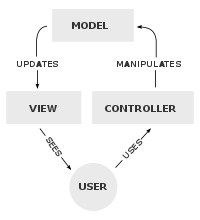
\includegraphics[width=0.6\textwidth]{sample_img.png}
  \caption{Hình ảnh mẫu sơ đồ hệ thống}
  \label{fig:sample}
\end{figure}

Như được thể hiện trên Hình \ref{fig:sample}, hệ thống gồm các thành phần cơ bản xử lý từ đầu vào đến kết quả trả về.

\subsection{Mục 2.1.2}
Phân tích thiết kế Cơ sở dữ liệu và các thành phần giao tiếp API.

% !TEX root = ../main.tex
\chapter{XÂY DỰNG VÀ KIỂM THỬ HỆ THỐNG}

\section{Mục 3.1}
Quá trình cài đặt và thực nghiệm hệ thống.

\begin{table}[htbp]
  \centering
  \caption{Bảng mẫu đánh giá kết quả thực nghiệm}
  \label{tab:sample}
  \begin{tabular}{|c|l|c|c|}
    \hline
    \textbf{STT} & \textbf{Tên tiêu chí}   & \textbf{Đơn vị} & \textbf{Kết quả} \\ \hline
    1            & Độ chính xác (Accuracy) & \%              & 94.5 \%          \\ \hline
    2            & Thời gian phản hồi      & giây            & 0.12 s           \\ \hline
    3            & Dung lượng bộ nhớ       & MB              & 45 MB            \\ \hline
  \end{tabular}
\end{table}

Bảng \ref{tab:sample} tổng hợp kết quả đo đạc các chỉ số hiệu năng của hệ thống.

\section{Mục 3.2}
Đánh giá mức độ hoàn thiện và khả năng đáp ứng yêu cầu bài toán.

% !TEX root = ../main.tex
\unchapter{KẾT LUẬN VÀ KIẾN NGHỊ}
Nêu kết luận cơ bản về những công việc đã thực hiện và hướng nghiên cứu cải tiến hệ thống đề xuất trong tương lai.



% ==============================================================================
% 6. Tài liệu tham khảo
% ==============================================================================
\cleardoublepage


\input{tailieuthamkhao.bib}

\end{document}
